\documentclass[compress]{beamer}
\usepackage{ifthen,verbatim}

\newcommand{\isnote}{}
\xdefinecolor{lightyellow}{rgb}{1.,1.,0.25}
\xdefinecolor{darkblue}{rgb}{0.1,0.1,0.7}

%% Uncomment this to get annotations
%% \def\notes{\addtocounter{page}{-1}
%%            \renewcommand{\isnote}{*}
%% 	   \beamertemplateshadingbackground{lightyellow}{white}
%%            \begin{frame}
%%            \frametitle{Notes for the previous page (page \insertpagenumber)}
%%            \itemize}
%% \def\endnotes{\enditemize
%% 	      \end{frame}
%%               \beamertemplateshadingbackground{white}{white}
%%               \renewcommand{\isnote}{}}

%% Uncomment this to not get annotations
\def\notes{\comment}
\def\endnotes{\endcomment}

\setbeamertemplate{navigation symbols}{}
\setbeamertemplate{headline}{\mbox{ } \hfill
\begin{minipage}{5.5 cm}
\vspace{-0.75 cm} \small
\end{minipage} \hfill
\begin{minipage}{4.5 cm}
\vspace{-0.75 cm} \small
\begin{flushright}
\ifthenelse{\equal{\insertpagenumber}{1}}{}{Jim Pivarski \hspace{0.2 cm} \insertpagenumber\isnote/\pageref{numpages}}
\end{flushright}
\end{minipage}\mbox{\hspace{0.2 cm}}\includegraphics[height=1 cm]{../cmslogo} \hspace{0.1 cm} \includegraphics[height=1 cm]{../tamulogo} \hspace{0.01 cm} \vspace{-1.05 cm}}

\begin{document}
\begin{frame}
\vfill
\begin{center}
\textcolor{darkblue}{\Large MC-Generated STARTUP Scenario}

\vfill
\begin{columns}
\column{0.3\linewidth}
\begin{center}
\large
\textcolor{darkblue}{Jim Pivarski}
\end{center}
\end{columns}

\begin{columns}
\column{0.3\linewidth}
\begin{center}
\scriptsize
{\it Texas A\&M University}
\end{center}
\end{columns}

\vfill
2 October, 2009

\end{center}
\end{frame}

%% \begin{notes}
%% \item This is the annotated version of my talk.
%% \item If you want the version that I am presenting, download the one
%% labeled ``slides'' on Indico (or just ignore these yellow pages).
%% \item The annotated version is provided for extra detail and a written
%% record of comments that I intend to make orally.
%% \item Yellow notes refer to the content on the {\it previous} page.
%% \item All other slides are identical for the two versions.
%% \end{notes}

\small

\begin{frame}
\frametitle{Motivation}
\begin{itemize}
\item The current muon misalignment scenarios (MC) are:
\begin{itemize}
\item STARTUP {\scriptsize (DTCRAFTScenario310\_v2\_mc and CSCCRAFTScenario310me42\_v2\_mc)}, produced by randomly misaligning chambers with an RMS consistent with cross-checks in CRAFT
\item 50 pb$^{-1}$ {\scriptsize (DT50InversepbScenario3XYv1\_mc and CSC50InversepbScenario3XYv1\_mc)}, produced by running the Reference-Target algorithm on appropriate MC samples
\end{itemize}

\item These are qualitatively different things: the latter includes internal correlations introduced by the procedure, the former does not
\end{itemize}

\vspace{0.2 cm}
\hspace{-0.83 cm} \textcolor{darkblue}{\Large What is presented here}

\begin{itemize}
\item MC-generated STARTUP DTAlignmentRcd
\begin{itemize}
\item tracker misalignment: produced by running the tracker alignment procedure on cosmics MC
\item DT misalignment: produced by running Reference-Target alignment on cosmics MC, using the above as input
\end{itemize}

\end{itemize}
\end{frame}

%% \section*{First section}
%% \begin{frame}
%% \begin{center}
%% \Huge \textcolor{blue}{First section}
%% \end{center}
%% \end{frame}

\begin{frame}
\frametitle{MC-generated STARTUP}
\begin{itemize}
\item Below: comparisons of muon chamber positions with MC truth
\begin{itemize}
\item $\delta_{x'}$, $\delta_{y'}$, $\delta_{z'}$ are local coordinates with consistent sign conventions
\end{itemize}
\item Aligned chamber positions are very sensitive to tracker misalignment
\end{itemize}

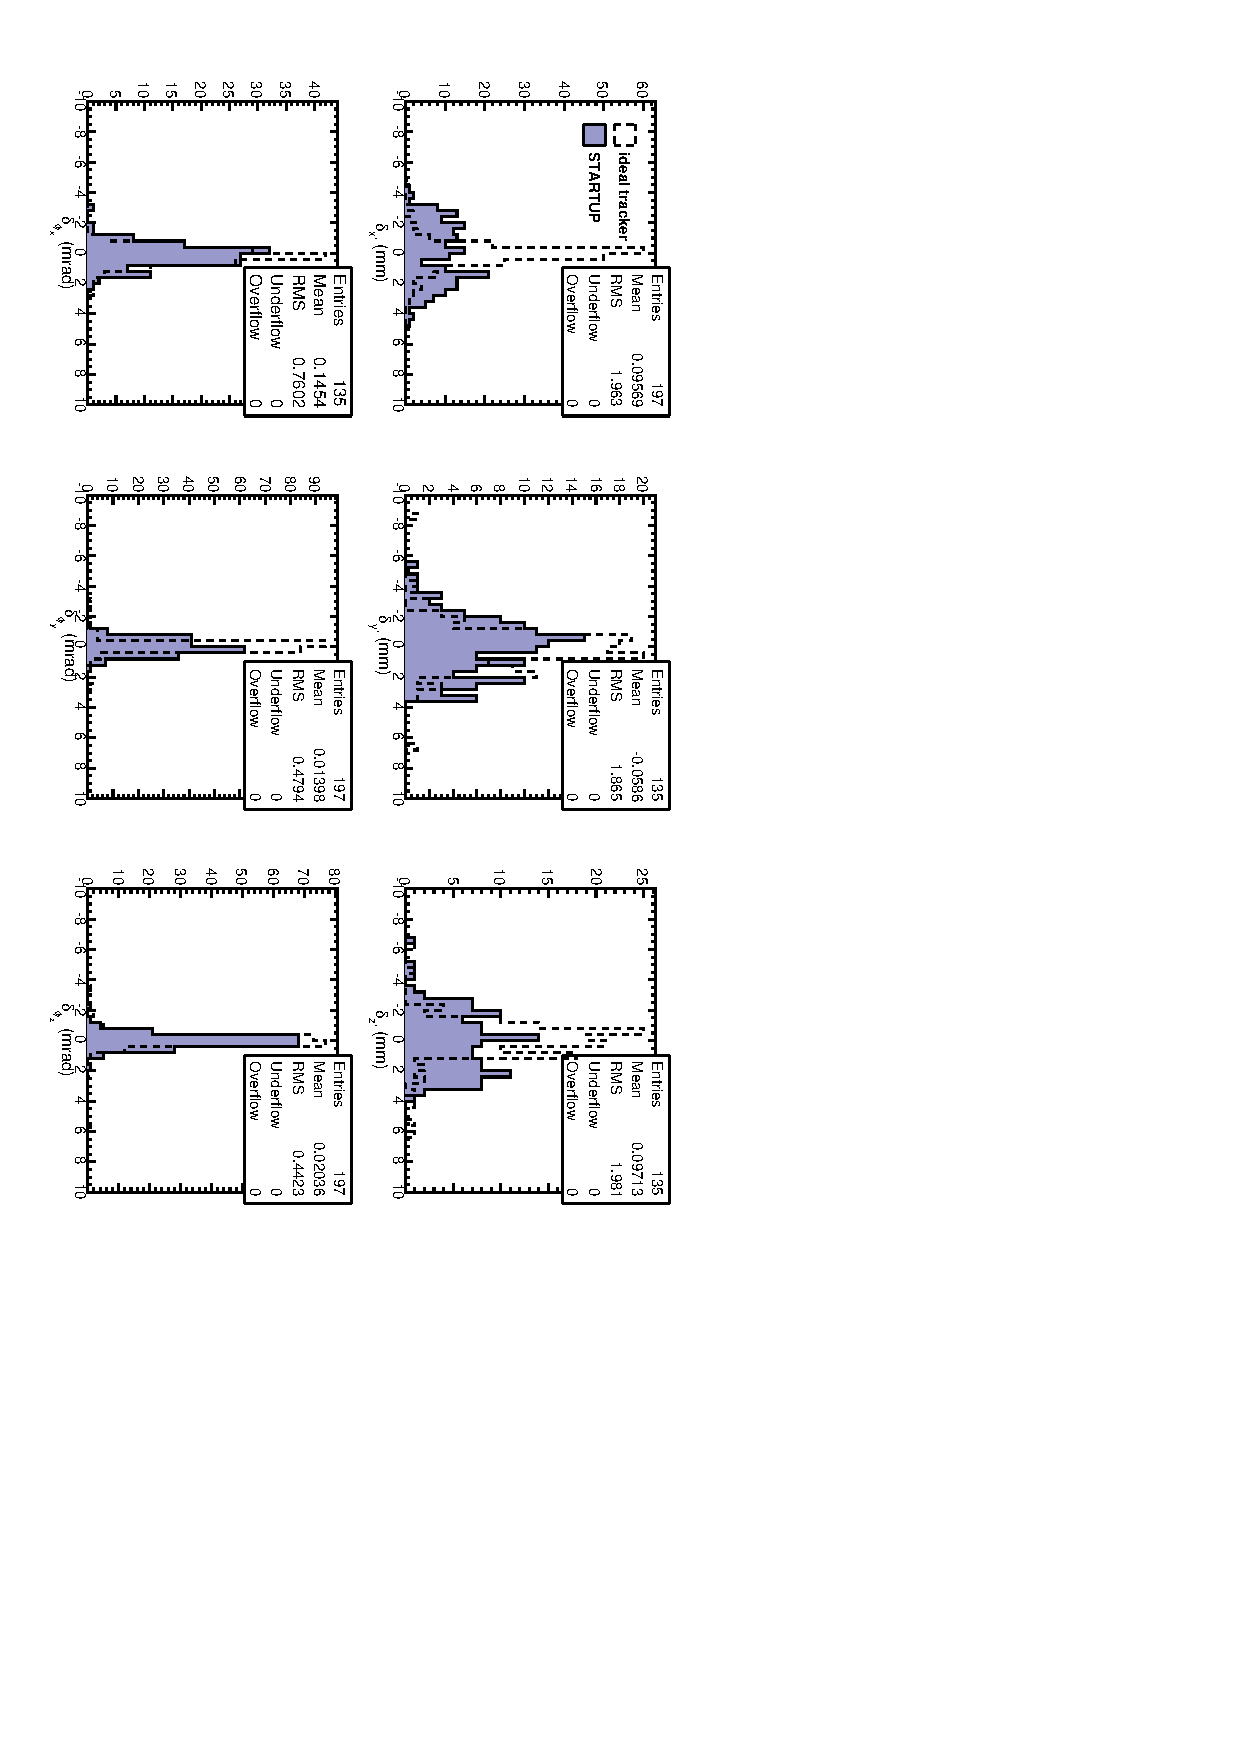
\includegraphics[height=0.95\linewidth, angle=90]{startup_6dof_redo.pdf}
\end{frame}

\begin{frame}
\frametitle{Tracker alignment systematics}
\framesubtitle{(Background for a muon systematics study on the following pages)}

\begin{itemize}
\item 9 cannonical modes: \{$R$, $z$, $r\phi$\} displacements vs.\ \{$R$, $z$, $\phi$\}
\item Left: tracker module positions in each mode
\end{itemize}

\begin{columns}
\column{0.5\linewidth}
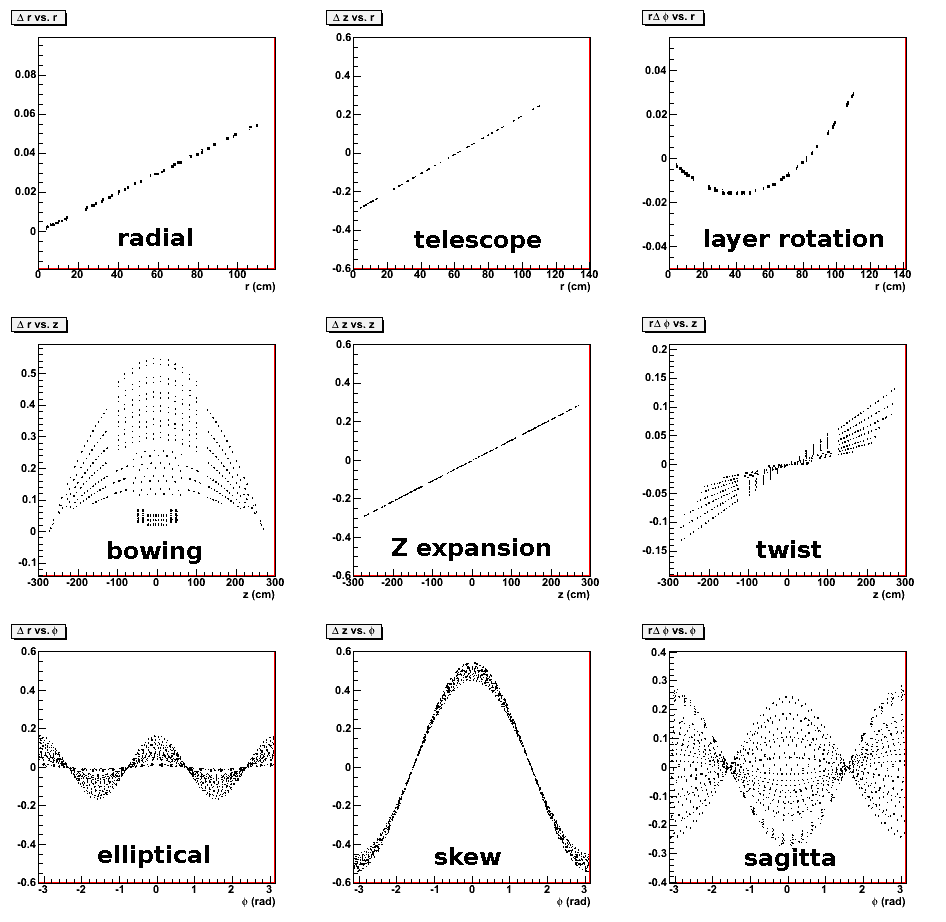
\includegraphics[width=\linewidth]{TrackerSystematics.png}
\column{0.5\linewidth}
\begin{itemize}
\item $\chi^2$ sensitivity of each mode
\item Cosmic rays are insensitive to \mbox{Z expansion}, skew, and sagitta
\end{itemize}

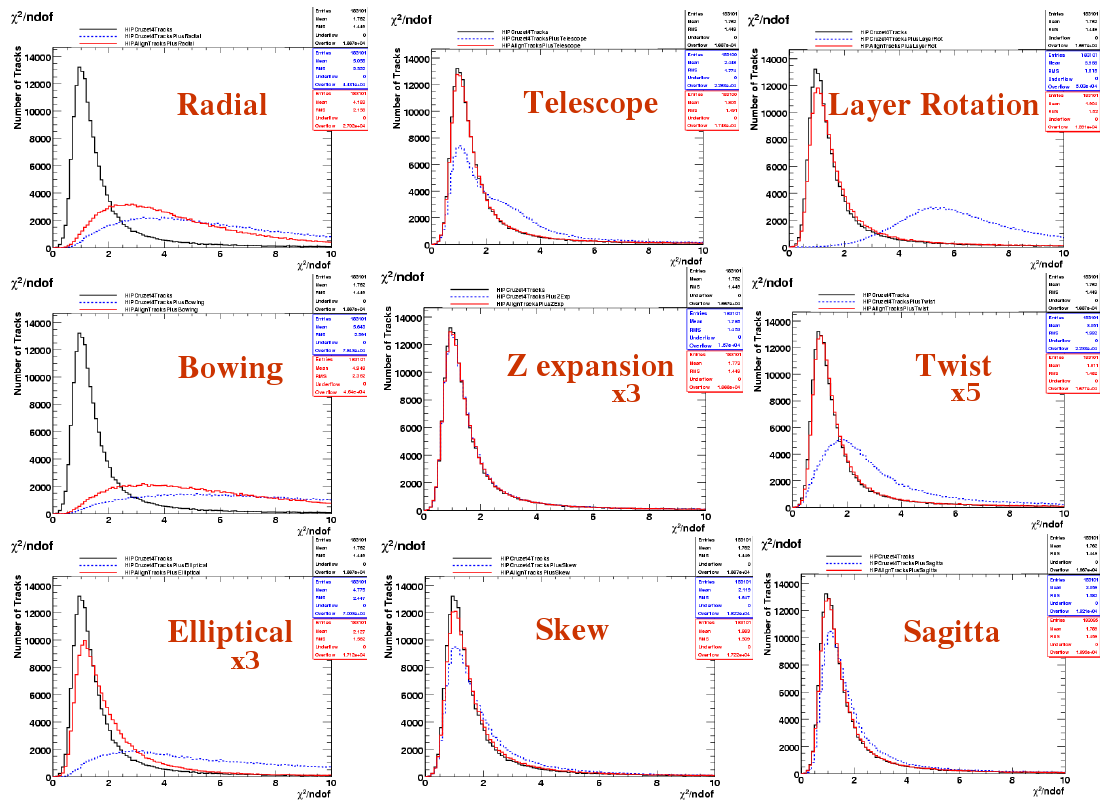
\includegraphics[width=\linewidth]{chi2_sensitivity.png}
\end{columns}
\end{frame}

\begin{frame}
\frametitle{Muon systematics study}
\framesubtitle{All plots are $\delta_\phi$ (rotation around beamline) versus $\phi$}
\begin{itemize}
\item Left: muon chamber positions in MC-generated STARTUP
\item Right: muon chamber positions for each cannonical tracker mode
\item STARTUP most resembles ``sagitta'' (10$\times$ smaller than cannonical)
\begin{itemize}
\item in cannonical scenarios, some chambers at extremes fail to fit
\end{itemize}
\end{itemize}

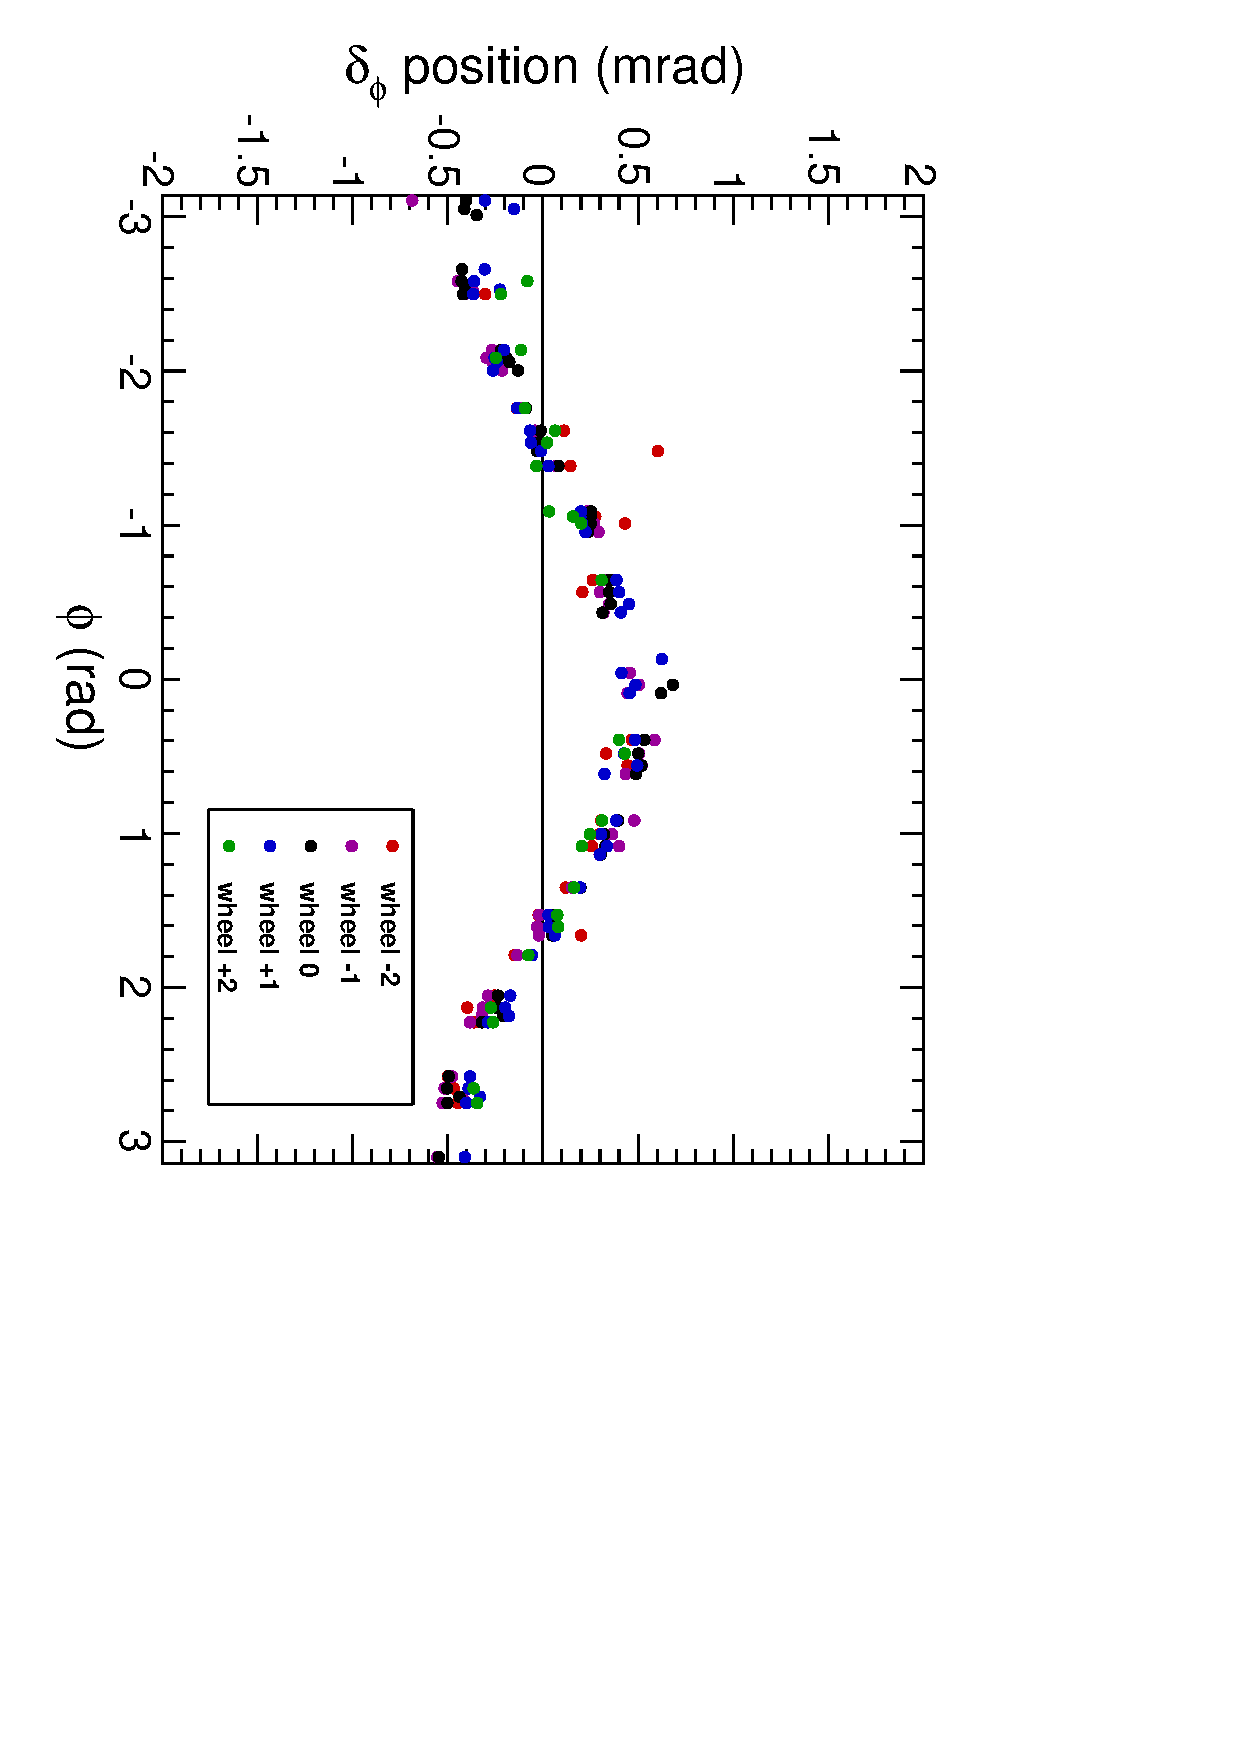
\includegraphics[height=0.5\linewidth, angle=90]{startup_phi_phi_redo.pdf}
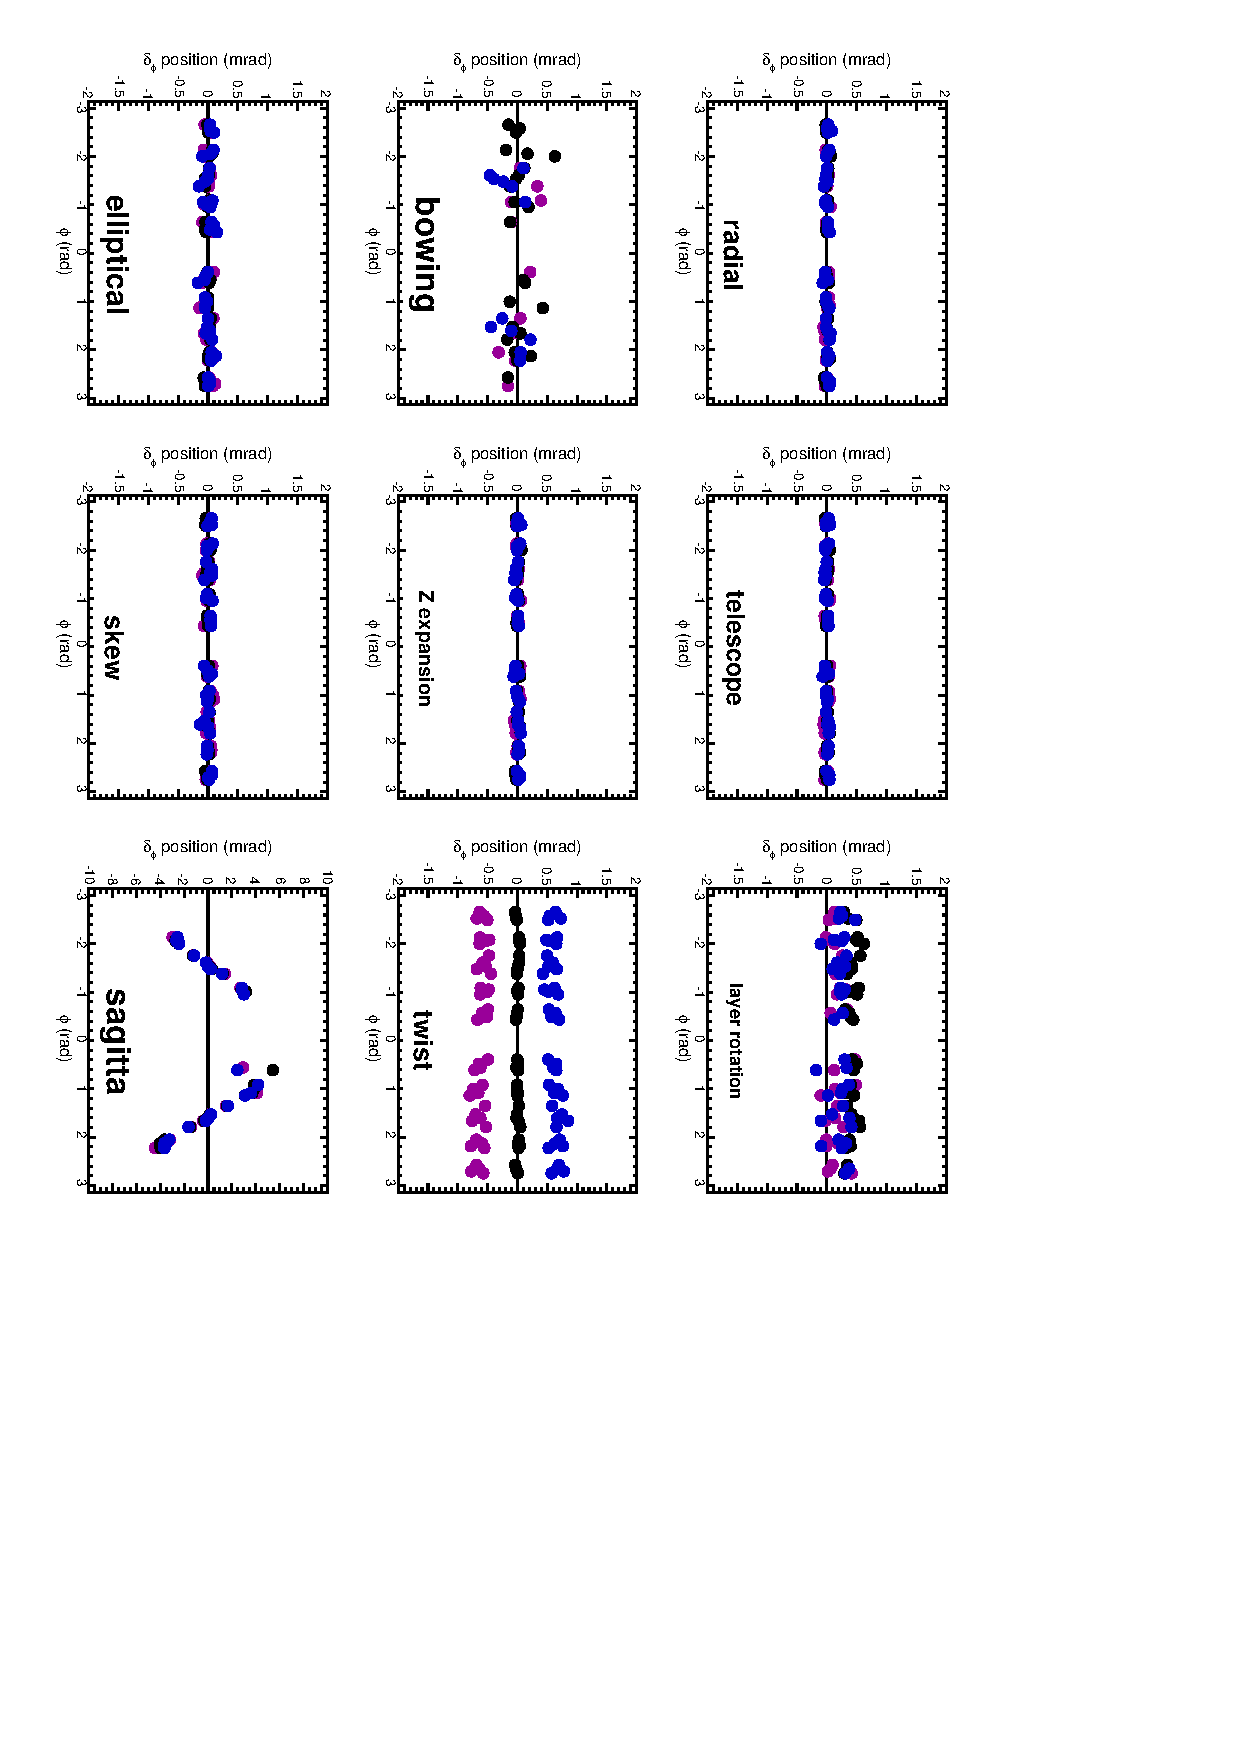
\includegraphics[height=0.5\linewidth, angle=90]{systematic_phi_phi_redo.pdf}
\end{frame}

\begin{frame}
\frametitle{Muon systematics study}
\framesubtitle{All plots are $\delta_{y'}$ (displacements parallel to beamline) versus $\phi$}
\begin{itemize}
\item Left: muon chamber positions in MC-generated STARTUP
\item Right: muon chamber positions for each cannonical tracker mode
\item STARTUP is not pure ``sagitta,'' but no sign of ``skew''
\end{itemize}

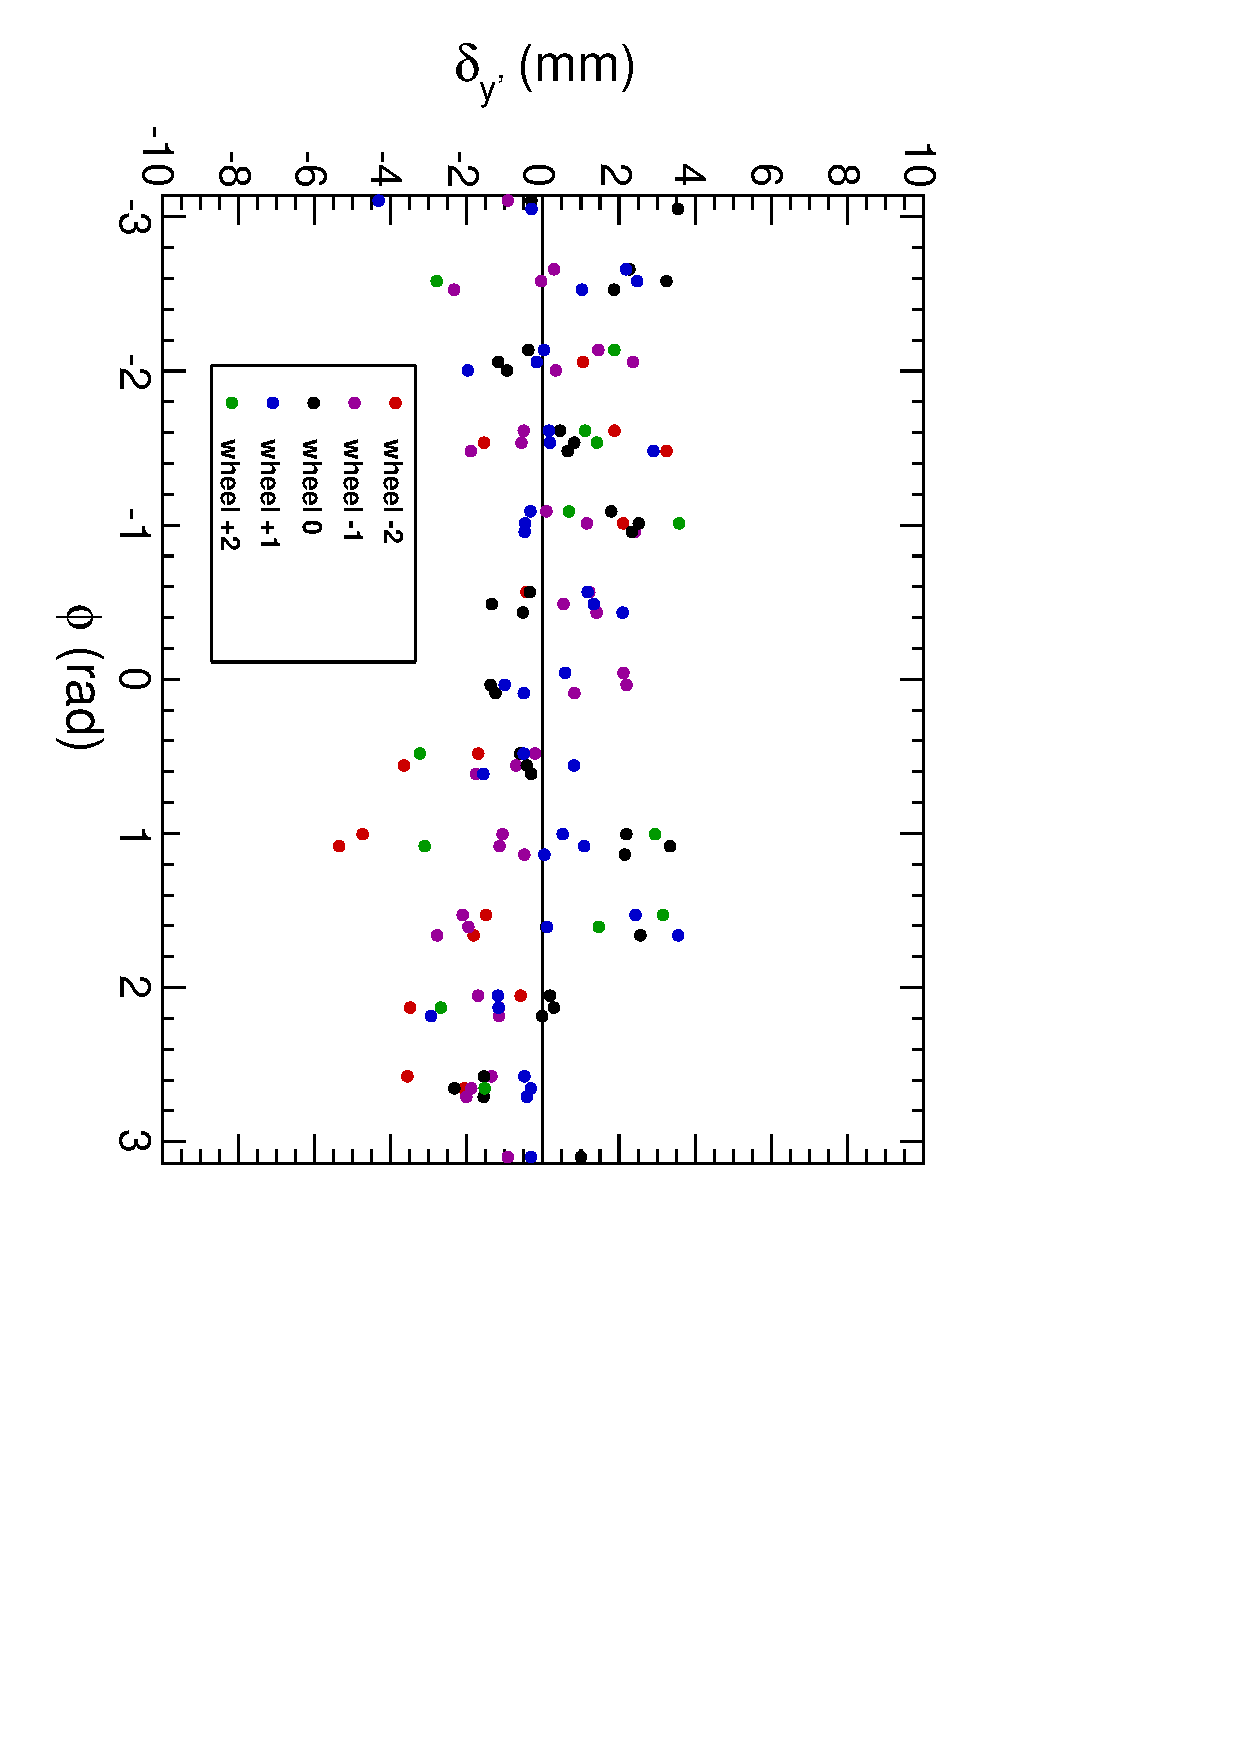
\includegraphics[height=0.5\linewidth, angle=90]{startup_y_phi_redo.pdf}
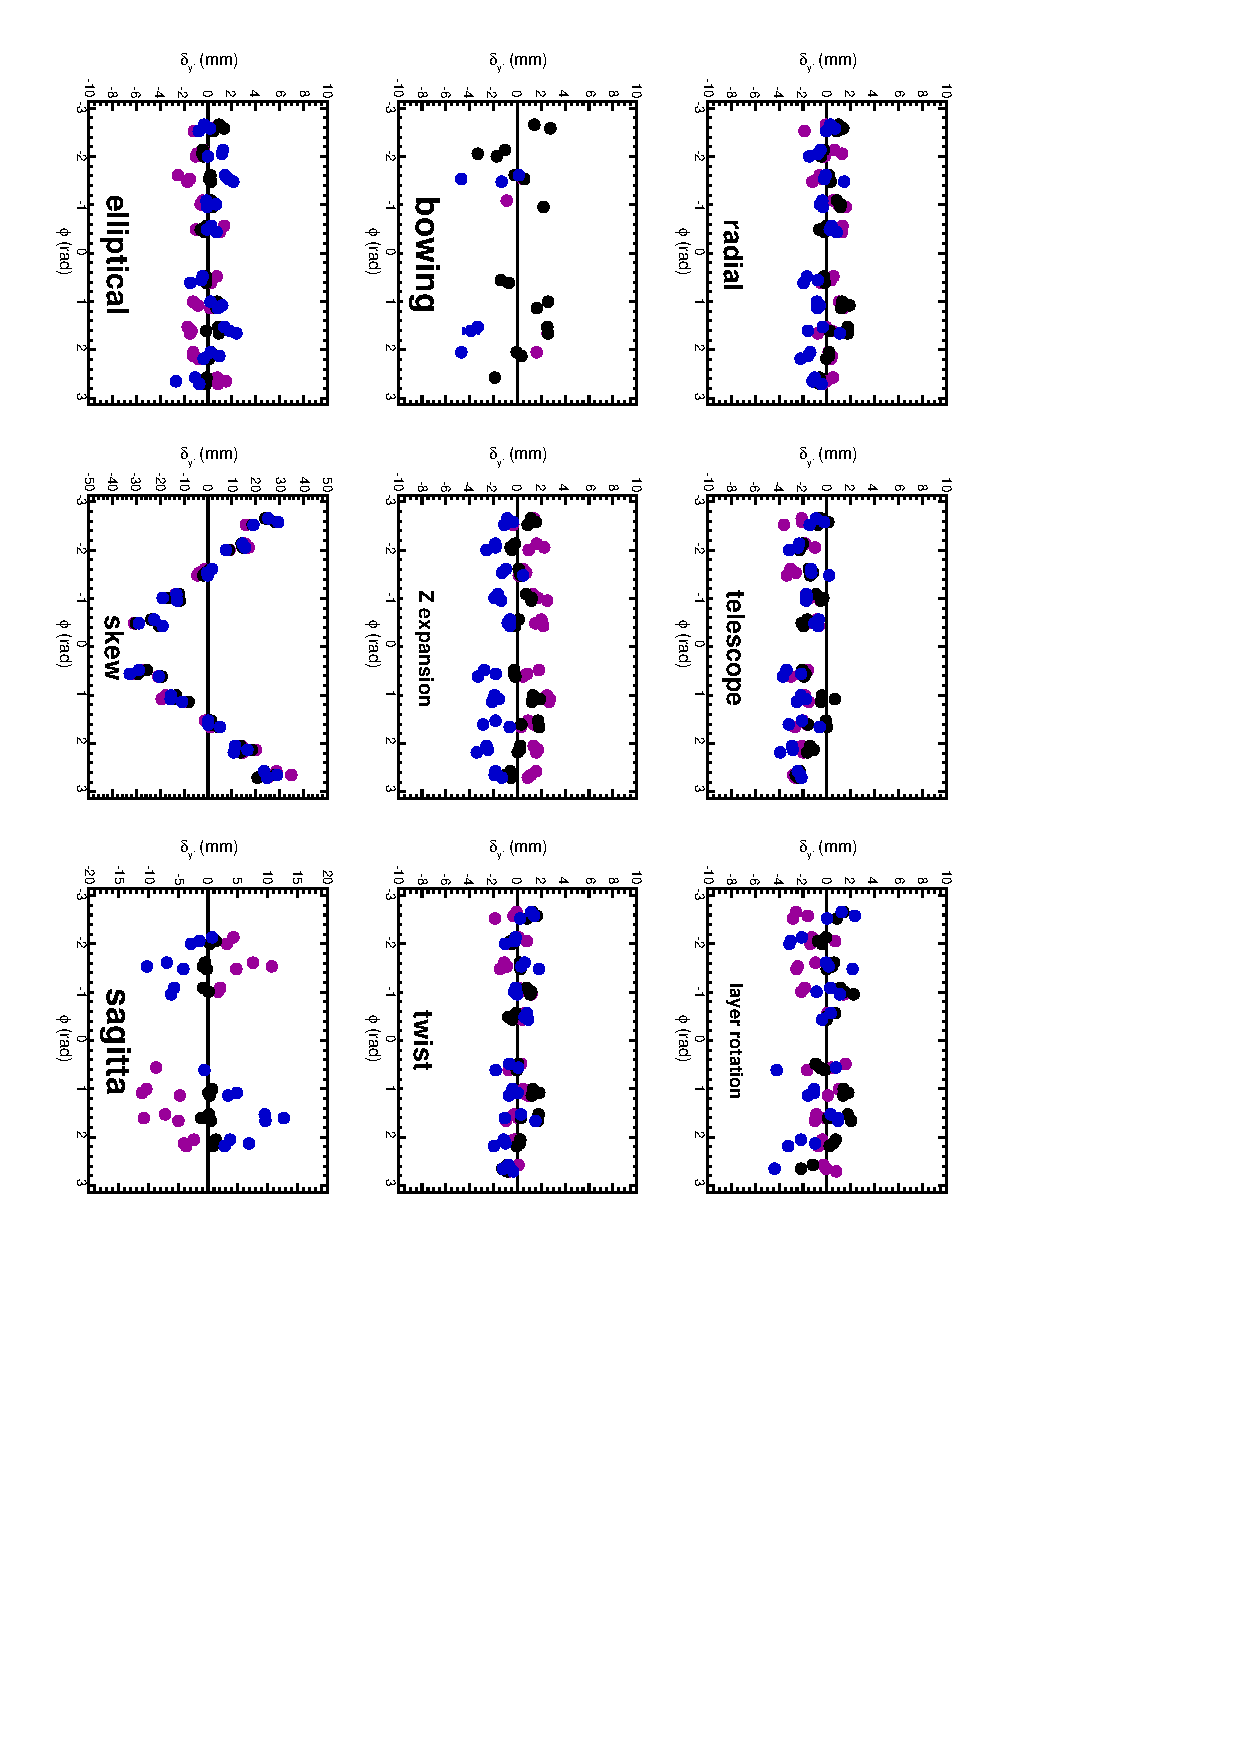
\includegraphics[height=0.5\linewidth, angle=90]{systematic_y_phi_redo.pdf}
\end{frame}

\begin{frame}
\frametitle{Muon systematics study}
\framesubtitle{All plots are $\delta_{z'}$ (radial displacements) versus $\phi$}
\begin{itemize}
\item Left: muon chamber positions in MC-generated STARTUP
\item Right: muon chamber positions for each cannonical tracker mode
\item We see the ``sagitta'' pattern dominating here, too
\end{itemize}

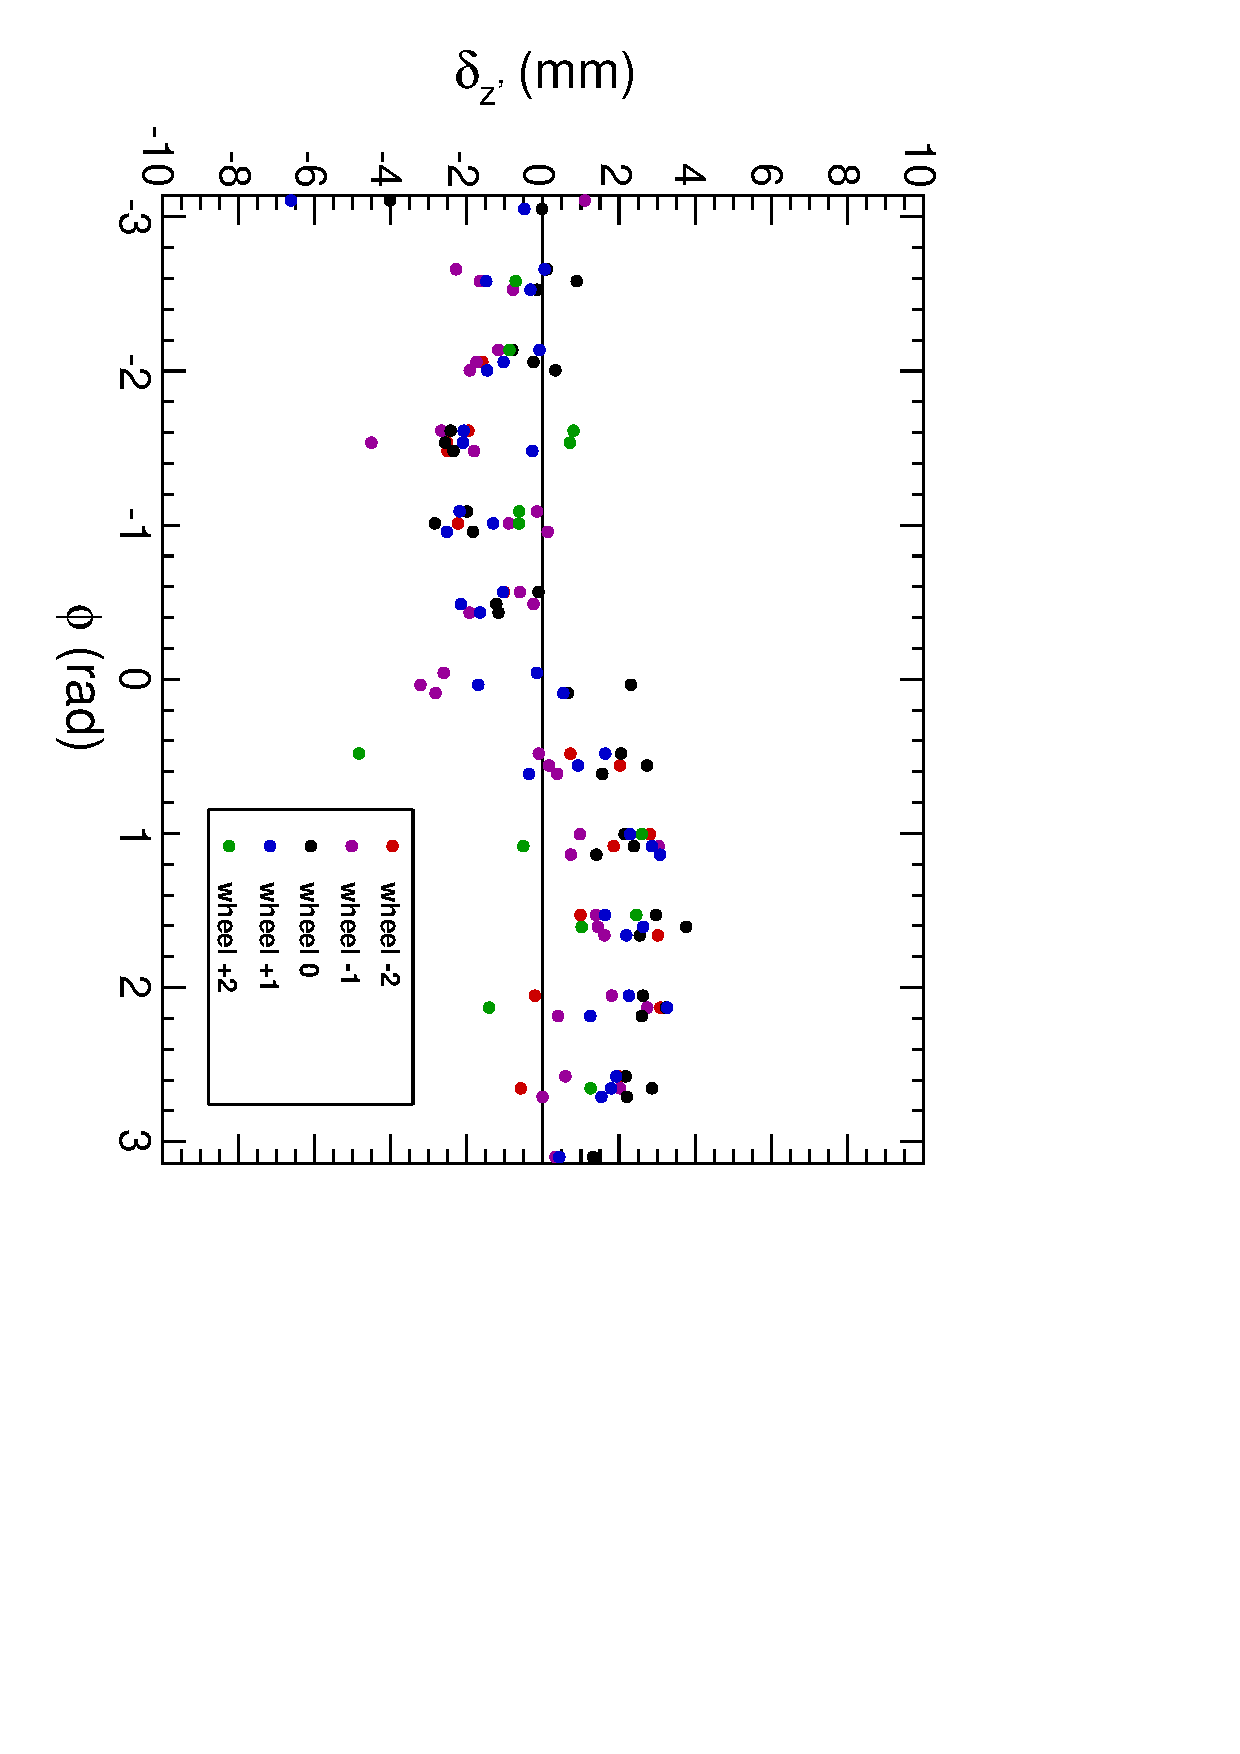
\includegraphics[height=0.5\linewidth, angle=90]{startup_z_phi_redo.pdf}
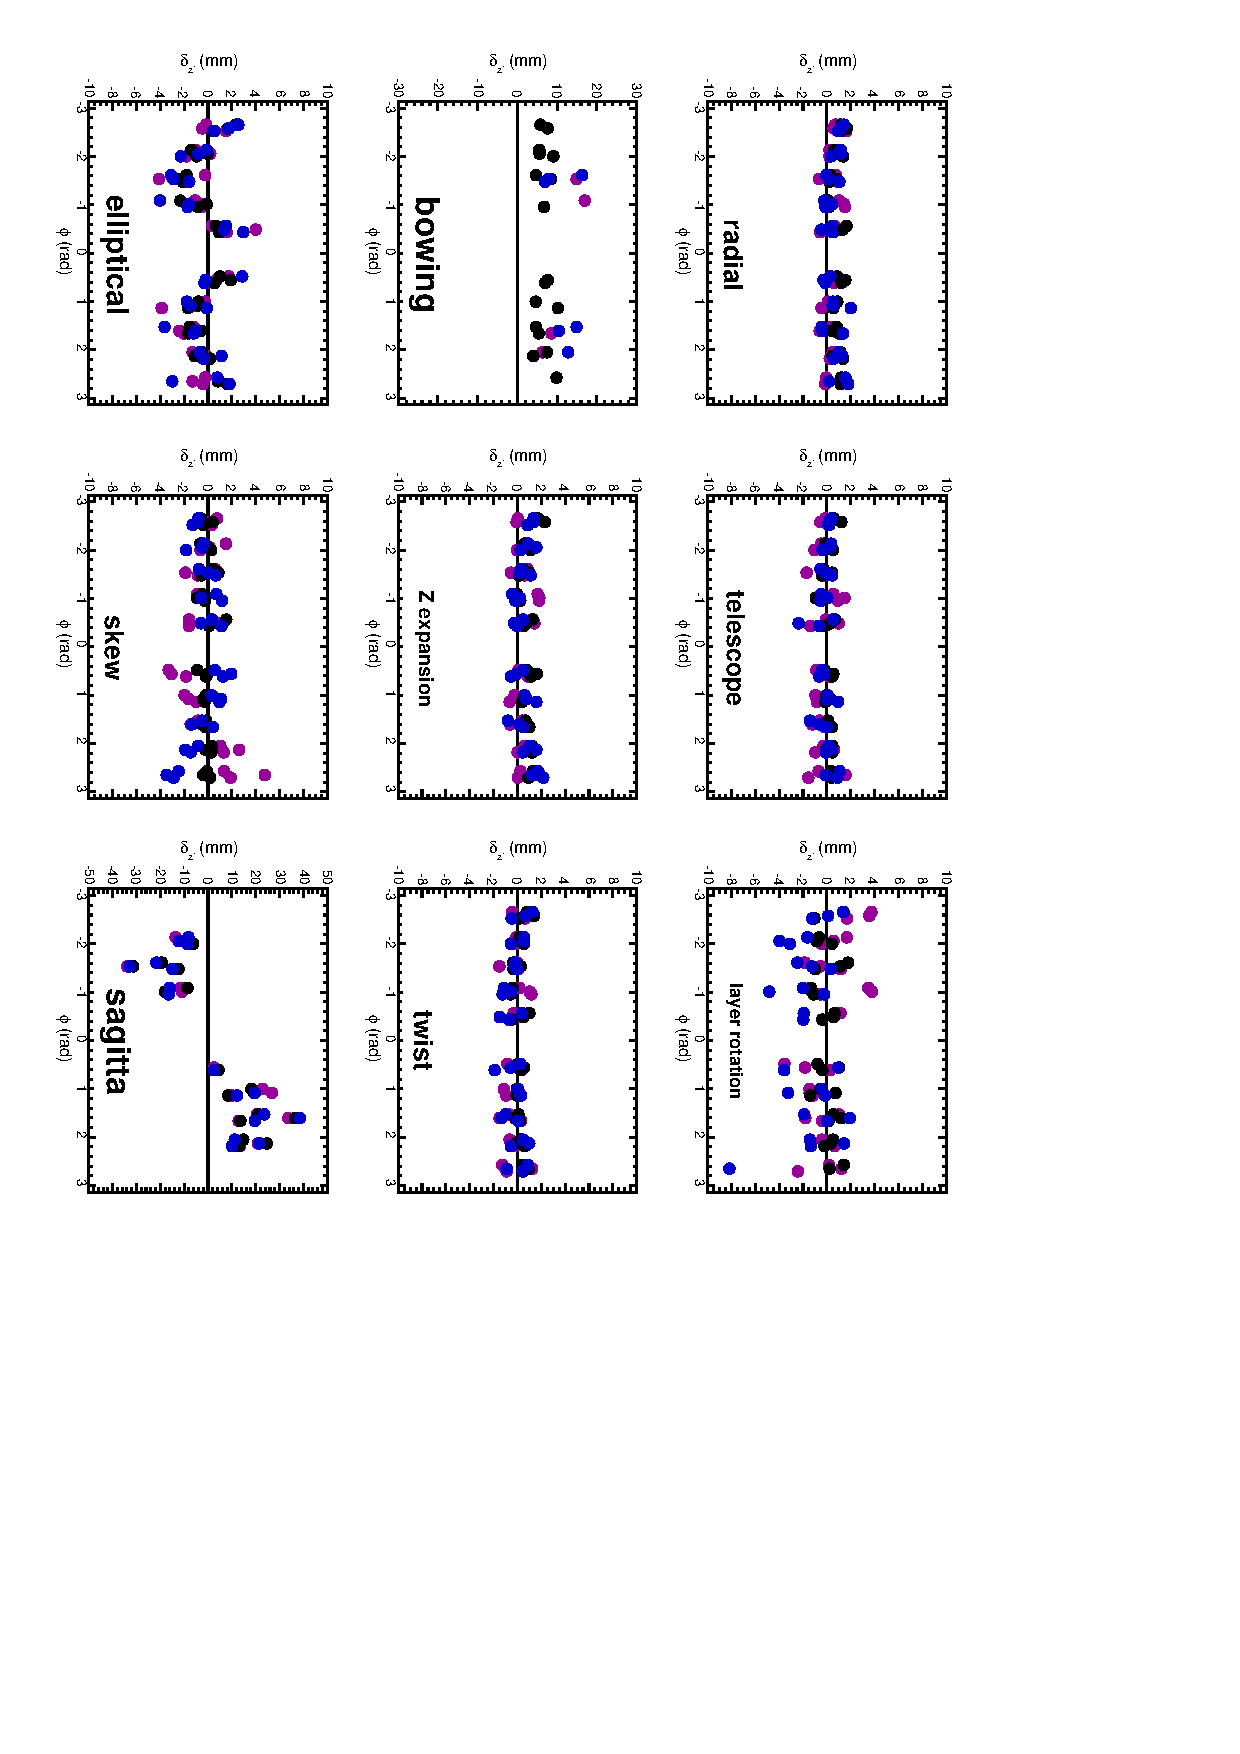
\includegraphics[height=0.5\linewidth, angle=90]{systematic_z_phi_redo.pdf}
\end{frame}

\begin{frame}
\frametitle{More tracker dependence}
\begin{itemize}
\item Final (official) tracker alignment differs from the first one we
  were given by a translation and rotation (centered on pixel instead
  of whole tracker)
\item Repeated muon alignment with final tracker alignment:
\begin{itemize}
\item {\it final} results shown on previous pages
\item difference between the two shown below, looks like a rotation around global Y ($\delta_{x'} \propto z \sin\phi$)
\end{itemize}

\end{itemize}
\begin{center}
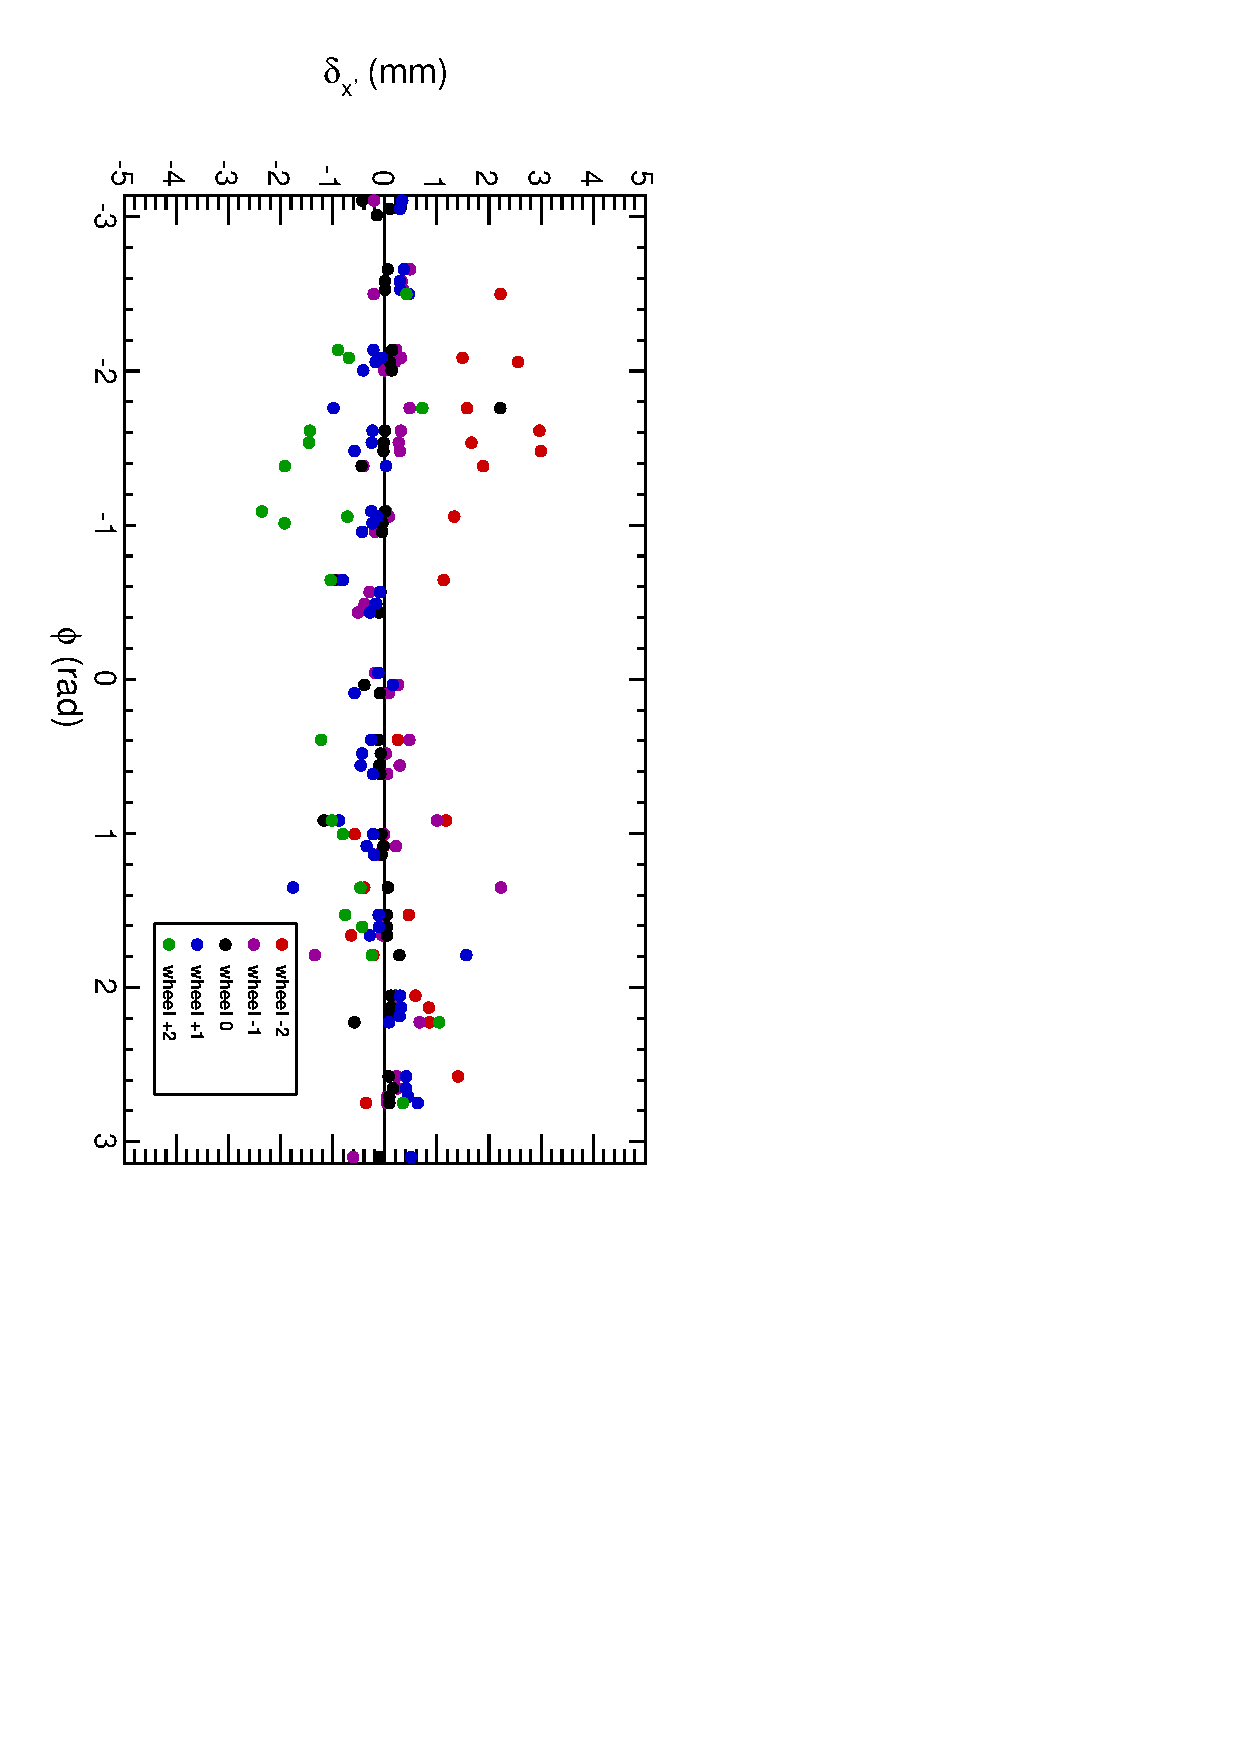
\includegraphics[height=0.8\linewidth, angle=90]{difference_of_tracker_centering3.pdf}
\end{center}
\end{frame}

\begin{frame}
\frametitle{Cosmic splitting validation}

\begin{itemize}
\item Vertical axis is $(\frac{q}{p_T}^{\mbox{\scriptsize top}} - \frac{q}{p_T}^{\mbox{\scriptsize bottom}})/(\sqrt{2} \frac{q}{p_T})$ for each split cosmic ray
\only<1>{\begin{itemize}
\item $10^{-1}$ means top-minus-bottom curvature difference is 10\% of the curvature {\scriptsize (and therefore $p_T$ error is approximately 10\% of $p_T$)}
\end{itemize}}
\item \scriptsize \textcolor{red}{COSMMC is random tracker, random muon}, \textcolor{green}{Jula-Zijin is MC-aligned tracker}, \textcolor{blue}{MCGeom + Jim's latest is MC-aligned tracker and muon}
\only<2>{\item ``TPFMS'' are track fits using the tracker and the first muon station}
\only<4>{\item Muon alignment has a small effect on tracker-only through the selection of tracks (globalMuon must be present to appear in this analysis)}
\end{itemize}

\begin{columns}
\column{0.83\linewidth}
\mbox{\hspace{0.5 cm}
\only<1>{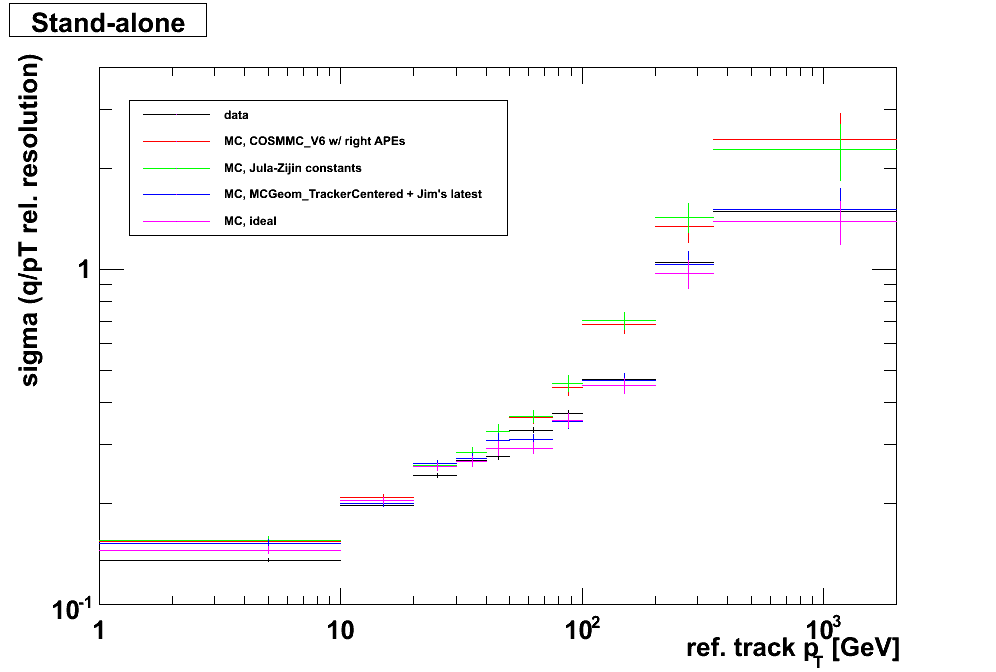
\includegraphics[width=\linewidth]{Stand-alone.png}}
\only<2>{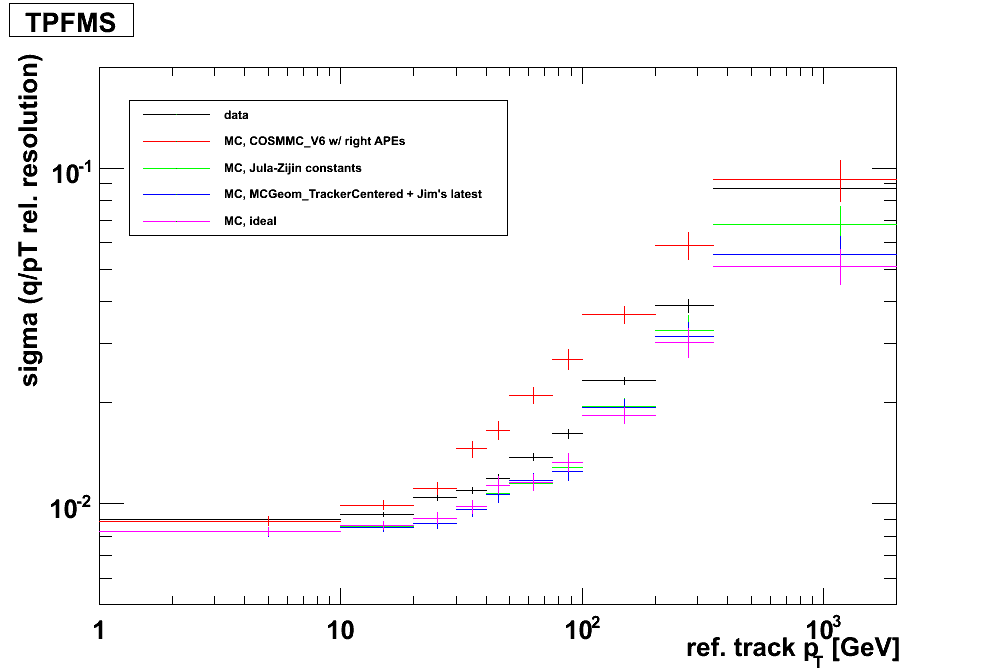
\includegraphics[width=\linewidth]{TPFMS.png}}
\only<3>{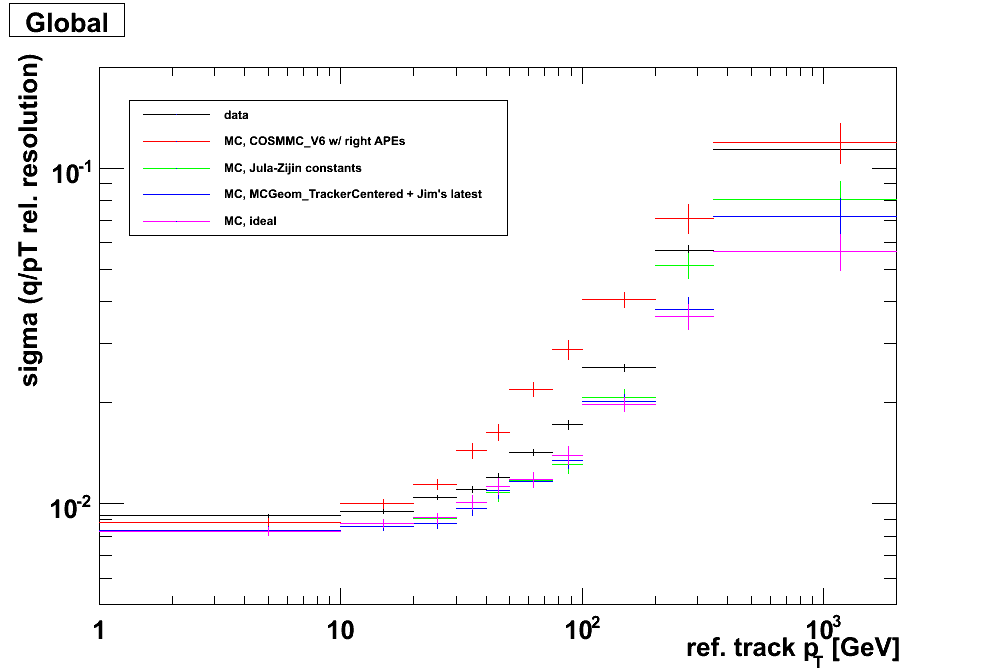
\includegraphics[width=\linewidth]{Global.png}}
\only<4>{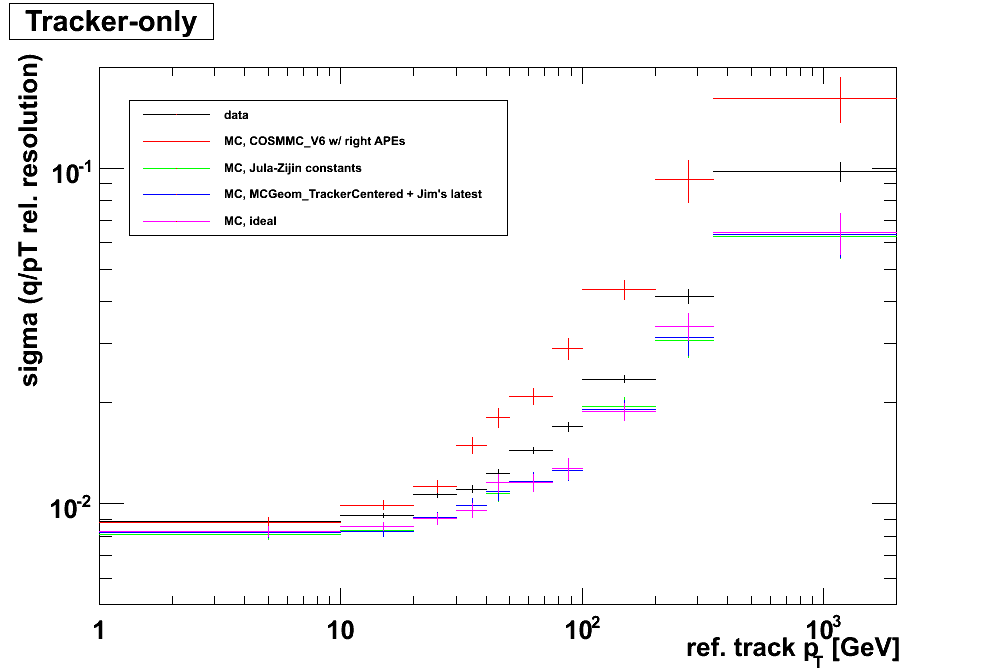
\includegraphics[width=\linewidth]{Tracker-only.png}}}

\column{0.25\linewidth}
\scriptsize
\textcolor{darkblue}{J.~Tucker}

\vspace{1 cm}
Non-final tracker alignment and non-final muon alignment, but mutually consistent

\vspace{2 cm}
\end{columns}
\end{frame}

\begin{frame}
\frametitle{DB comparison conclusions}
\begin{itemize}
\item MC-generated tracker misalignment is globally distorted
\item We've characterized the muon alignment's response to all of the cannonical global distortions: this one is ``sagitta'' (not surprising: tracker $\chi^2$ is insensitive to sagitta distortions in cosmic rays)
\item Near-ideal momentum resolution with a systematically-distorted tracker and muon system: an example of an ``effective detector''
\end{itemize}

\vspace{0.2 cm}
\hspace{-0.83 cm} \textcolor{darkblue}{\Large Cosmic splitting conclusions}
\begin{itemize}
\item MC-generated scenarios underestimate resolution, related to unmodeled detector effects in alignment step or track-fitting
\item But MC now has a more similar shape as a function of $p_T$
\item Ideal MC agrees with PTDR Figure~1.5 ($(p^{\mbox{\scriptsize reco}} - p^{\mbox{\scriptsize gen}})/p^{\mbox{\scriptsize gen}}$ in $0 < \eta < 0.2$) and tracker-only agrees with Nhan's analysis ($p_T$ instead of $q/p_T$)
\item Tracker $+$ first muon station is only a little better than tracker-only in the highest bin (5.5\% vs.\ 6\%), similar to what we see in data (9\% vs.\ 10\%)
\end{itemize}
\end{frame}

\begin{frame}
\frametitle{Currently in the database}
\begin{itemize}
\item MC-generated tracker scenario approved and uploaded as TrackerAlignment\_CRAFT08Realistic\_mc
\begin{itemize}
\item intended to become new STARTUP scenario, but not in any globalTags yet
\end{itemize}
\item Current DTAlignmentRcd: randomly-generated constants whose scale is based on CRAFT validation
\item Current CSCAlignmentRcd: randomly-generated constants whose scale is based on hardware validation
\end{itemize}

\vspace{0.2 cm}
\hspace{-0.83 cm} \textcolor{darkblue}{\Large Recommendation}
\begin{itemize}
\item Upload MC-generated DTAlignmentRcd/DTAlignmentErrorRcd
\item Combine MC-generated tracker, MC-generated DT, and hardware estimated CSC into one globalTag
\begin{itemize}
\item asymmetry between DT and CSC is related to the fact that they're handled differently with cosmic rays, and this is a STARTUP scenario
\end{itemize}
\end{itemize}
\end{frame}

\begin{frame}
\frametitle{Where to find them}

{\tt \tiny
/afs/cern.ch/user/p/pivarski/public/DTAlignmentRcd\_cosmics-finaltracker\_22X\_v1.db

/afs/cern.ch/user/p/pivarski/public/DTAlignmentRcd\_cosmics-finaltracker\_3XY\_v1.db

/afs/cern.ch/user/p/pivarski/public/DTAlignmentRcd\_cosmics-finaltracker\_v1.xml}

\vfill

``22X'' is only compatible with 22X, ``3XY'' is only compatible with 3XY

\vfill

Usual tagnames: ``DTAlignmentRcd'' and ``DTAlignmentErrorRcd'' (ignore the CSCAlignmentRcd/CSCAlignmentErrorRcd)

\vfill
``DTAlignmentErrorRcd'' masks out unaligned chambers

\label{numpages}
\end{frame}

\end{document}
